\documentclass[dvipdfmx,11pt]{beamer}
\usepackage{lipsum}
\usetheme{EastLansing}
\usepackage{bxdpx-beamer}
\usepackage{pxjahyper}
\usepackage{minijs}
\usepackage{mathpazo}
\usepackage{amsmath,amssymb}
\usepackage{graphicx}
\usepackage{array}
\usepackage{tikz}
\usepackage{wrapfig}
\usepackage{float}
\usepackage{here}
\usepackage{lscape}
\usepackage{siunitx}
\setbeamertemplate{navigation symbols}{}

\title{Productivity effects of air pollution: \\ Evidence from professional soccer}
\subtitle{Lichter, Pestel and Sommer: (2017, Labour Economics)}
\author{Reio TANJI}
\date{May 23th, 2020}
\institute{Osaka University, Graduate School of Economics}

\begin{document}
\begin{frame}\frametitle{}
\titlepage
\end{frame}

\section{Introduction}

\begin{frame}\frametitle{Abstract}
  \begin{itemize}
    \item Research Question
    \begin{itemize}
      \item How large is the causal effect of ambient air pollution on individual productivity?
      \item If so, do individuals take optimization and avoidance behavior?
    \end{itemize}
    \item Strategy
    \begin{itemize}
      \item Panel data on the professional soccer players in Germany
    \end{itemize}
    \item Results
    \begin{itemize}
      \item An increase in the concentration of particulate matter reduces the total number of total passes played.
      \item In response, players adjust their effort provision.
    \end{itemize}
  \end{itemize}
\end{frame}

\begin{frame}\frametitle{Literature and Contribution}
  \begin{itemize}
    \item Air pollution is considered an important environmental risk factor for human health.
    \begin{itemize}
      \item Exposure to air pollution causes more than 550,000 premature deaths per year in Europe (EEA, 2016).
      \item A vast number of epidemiological studies to assess the health impacts of air pollution.
    \end{itemize}
    \item Economics: highlights the importance of individuals' optimization and avoidance behavior in response to to air pollution
    \begin{itemize}
      \item In addition to causing damage to individuals health, ambient air pollution may induce additional costs for societies by reducing individuals' labor supply and productivity.
    \end{itemize}
    \item This paper contributes by analyzing the effect of ambient air pollution on the productivity of young adults: positively selected with respect to their general physiological condition.
  \end{itemize}
\end{frame}

\section{Background and Data}

\begin{frame}\frametitle{Background and Confirmation of Exogeneity}
  \begin{itemize}
    \item \textit{Bundesliga}
    \begin{itemize}
      \item Germany's top professional league of men's soccer.
      \item A season comprises 34 matchdays and 306 matches (18 teams $\times$ 2 matches)
      \item Games are typically held on weekends between late August ad May.
      \item Schedules are beyond any control of teams and players because the League determines when and where the match is held.
      \begin{itemize}
        \item Individual exposure to ambient air pollution can be considered exogeneous.
      \end{itemize}
    \end{itemize}
    \item Merging this with an hourly data on the concentration of particulate matter (PM10) and ozone ($O_3$) at the time of kick-off
    \begin{itemize}
      \item PM10 is harmful to humans' health as it affects the pulmonary and cardiovascular functioning.
      \item Ozone impede the respiratory system of the human body.
    \end{itemize}
  \end{itemize}
\end{frame}

\begin{frame}\frametitle{}
  \begin{figure}
    \centering
    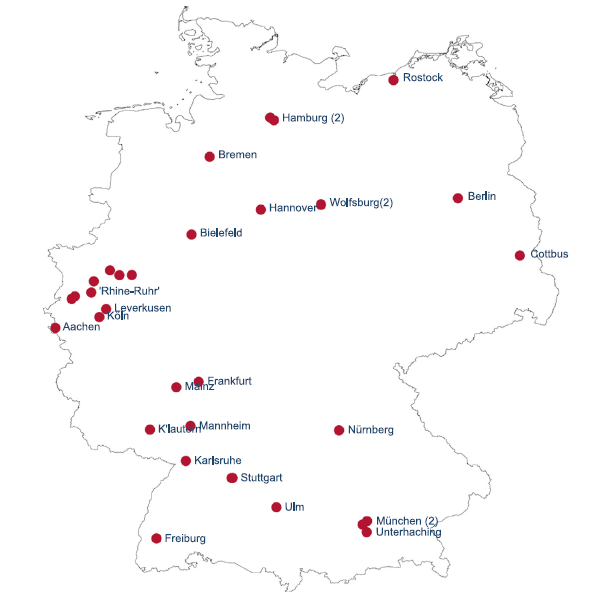
\includegraphics[scale = .7]{0522tanji_fig/f1}
    \label{f1}
  \end{figure}
\end{frame}

\begin{frame}\frametitle{Data}
  \textbf{Productivity of soccer players}
  \begin{itemize}
    \item \textbf{deltatre}
    \begin{itemize}
      \item provides information on player's productivity
      \item A commercial enterprise collecting data on professional sports and serving as and external service provider to the media and sports clubs.
    \end{itemize}
    \item Information on all the matches for every season from 1999/2000 to 2010/2011.
    \begin{itemize}
      \item \textbf{match}: location, date and kick-off time, home and away teams
      \item \textbf{player}: who was on the pitch at any poiny during the match.
    \end{itemize}
    \item $N = 75,163$ (1771 professional athletes $\times$ 2956 matches).
    \begin{itemize}
      \item 29 different teams in 32 stadiums during 1999/2000 - 2010/2011 seasons
    \end{itemize}
  \end{itemize}
\end{frame}

\begin{frame}\frametitle{}
  \begin{itemize}
    \item Proxy for individual productivity: \textbf{Players' total \# of passes}
    \begin{itemize}
      \item serves as on key statistic for the assesment of players' performance in soccer matches.
      \item A team's number of completed passes significantly increases just before scoring (Redwood-Brown, 2008)
      \item A strong positive relationship between the \# of passes and various measures of team success (Collet, 2013)
    \end{itemize}
    \item Additional measures: \textbf{pass accuracy} and \textbf{ratio of long over short passes}
    \begin{itemize}
      \item The former reflects players' \textbf{physical ability}, and the latter represents a \textbf{behavioral response} in the players' style of play.
    \end{itemize}
  \end{itemize}
  \begin{figure}
    \centering
    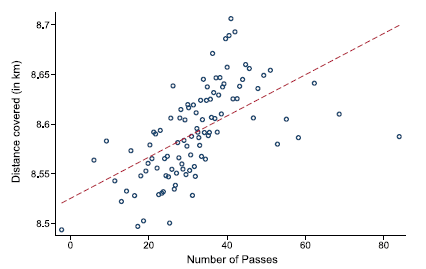
\includegraphics[scale = .5]{0522tanji_fig/fa1}
    \label{fa1}
  \end{figure}
\end{frame}

\begin{frame}\frametitle{}
  \textbf{Air pollution and weather}
  \begin{itemize}
    \item \textit{German Federal Environment Agency}
    \begin{itemize}
      \item Hourly monitor readings for the concentration of pollutants
      \begin{itemize}
        \item PM10: particulates with a diameter smaller than ten micrometers.
        \item Ozone: impede the respiratory system of the human body.
      \end{itemize}
      \item They computed inverse-distance weighted means of them, for each stadium the match was held.
      \begin{itemize}
        \item Matches without pullution readings within this radius are dropped (716 out of 3672)
      \end{itemize}
    \end{itemize}
    \item \textit{German Meteorological Service}
    \begin{itemize}
      \item Supplimental weather conditions: daily temperature, precipitation, humidity, air pressure, and wind speed.
    \end{itemize}
  \end{itemize}
\end{frame}

\begin{frame}\frametitle{Descriptive statistics}
  \begin{figure}
    \centering
    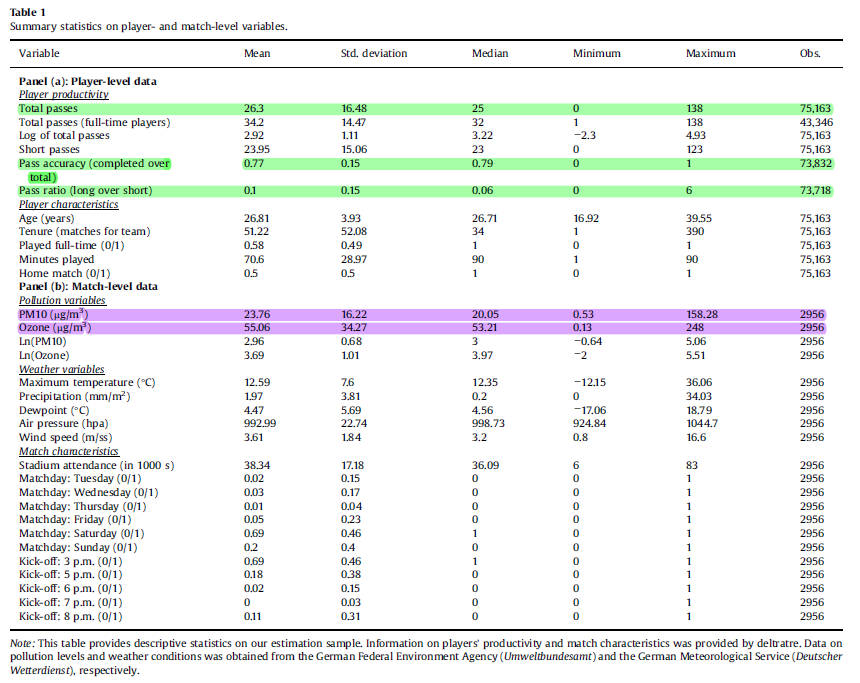
\includegraphics[scale = .6]{0522tanji_fig/t1}
    \label{t1}
  \end{figure}
\end{frame}

\begin{frame}\frametitle{}
  \begin{figure}
    \centering
    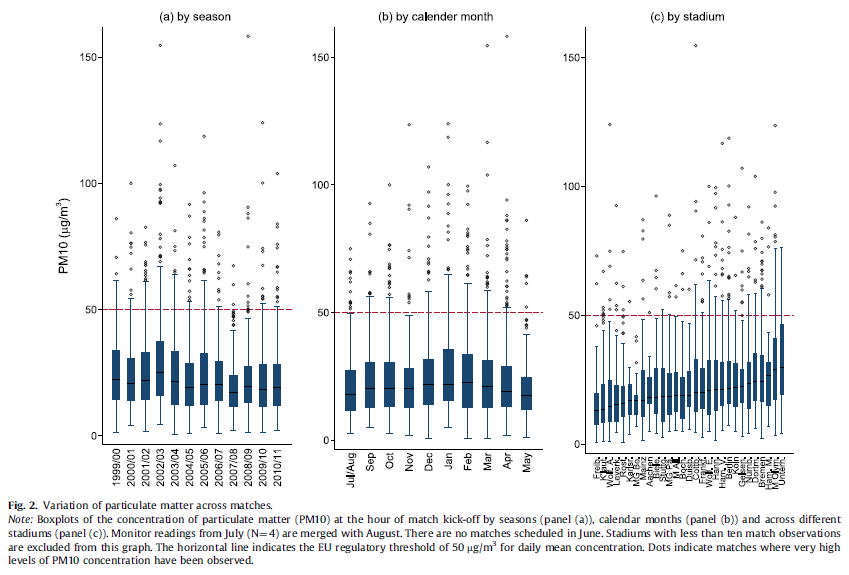
\includegraphics[scale = .8]{0522tanji_fig/f2}
    \label{f2}
  \end{figure}
\end{frame}

\begin{frame}\frametitle{}
  \begin{figure}
    \centering
    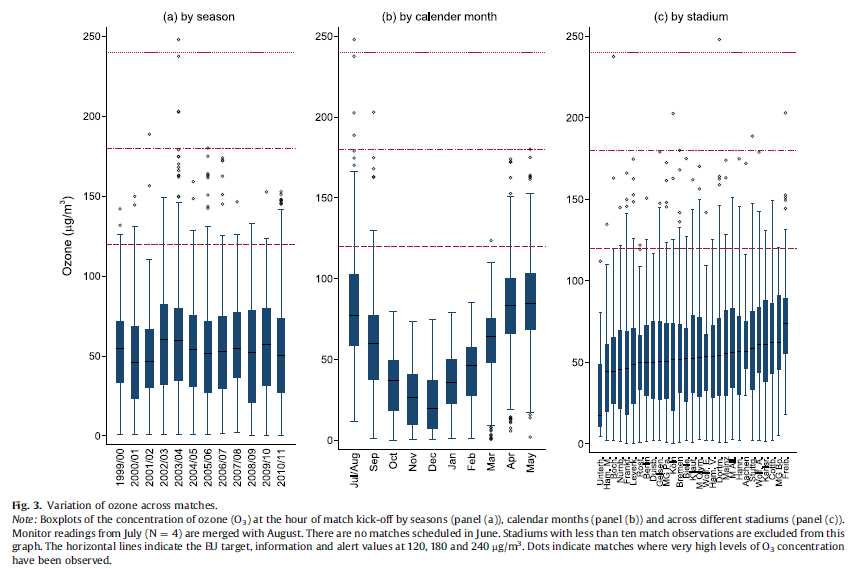
\includegraphics[scale = .8]{0522tanji_fig/f3}
    \label{f3}
  \end{figure}
\end{frame}

\section{Empirical Strategy}

\begin{frame}\frametitle{Empirical Strategy}
  \begin{align*}
    \text{Passes}_{imt} = & \beta_1 \text{PM10}_m + \beta_2 \text{Ozone}_m + X'_{imt}\gamma + W'_m \delta + M'_m \mu \\
    & + C_{c(tm)} + T_{ts(m)} \alpha_i + \epsilon_{imt}
  \end{align*}
  \begin{itemize}
    \footnotesize
    \item player $i$ in match $m$ for team $t$.
    \item The coefficients of interest: $\beta_1$ and $\beta_2$.
    \item $X_{imt}$ : individual player characteristics and dummy for home team.
    \item $W_m$: weather condition (standardized and entered in linear and quadratic form)
    \item $M_m$: match-specific features; day of the week, kick-off time and stadium attendance.
    \item $C$, $T$: coach and team-by-season fixed effects, respectively.
    \item Standard errors are clustered at the match level.
  \end{itemize}
\end{frame}

\section{Results}

\begin{frame}\frametitle{Results}
  \begin{figure}
    \centering
    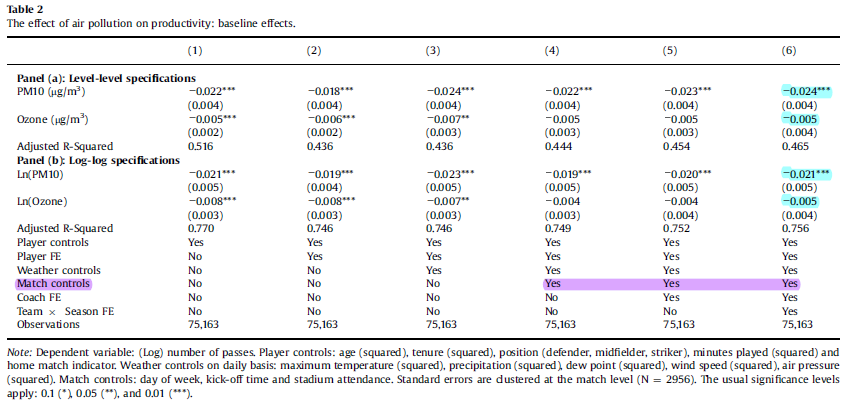
\includegraphics[scale = .7]{0522tanji_fig/t2}
    \label{t2}
  \end{figure}
\end{frame}

\begin{frame}\frametitle{Baseline}
  \begin{itemize}
    \item Statistically sigificant negative effects of both PM10 and ozone on players's productivity.
    \begin{itemize}
      \item One-standard deviation increase in PM10 concentration (roughly  \SI{16}{\micro g/m^3}) lowers passes by around 2.4\% of a standard deviation on average.
      \item 1\% increase in concentration reduces passes by .021\%.
    \end{itemize}
    \item By contrast, the effect of ozone is limited: variation in ozone concentration in the sample is limited.
    \begin{itemize}
      \item Only a tiny number of matches taked place during June or July.
    \end{itemize}
  \end{itemize}
\end{frame}

\begin{frame}\frametitle{Different marginal effect}
  \begin{itemize}
    \small
    \item Non-linear dose-response relationship
    \begin{itemize}
      \footnotesize
      \item \textbf{Kernel-weighted} local fourth-order polynomial regression
      \item Regression of match-level PM10 concentration on players' total passes without any further controls.
    \end{itemize}
    \item Based on this evidence, they tried linear regression again, allowing for different marginal effects below and above the identified thresholds.
    \begin{itemize}
      \footnotesize
      \item The negative effect becomes larger for PM10 levels around \SI{55}{\micro g/m^3} and above, although differences are not statistically insignificant.
    \end{itemize}
  \end{itemize}

  \begin{figure}
    \centering
    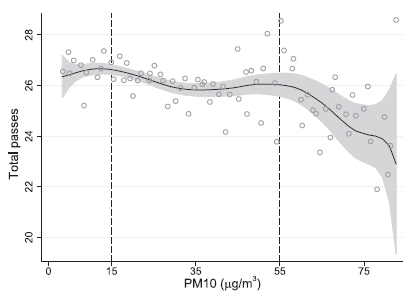
\includegraphics[scale = .7]{0522tanji_fig/f4}
    \label{f4}
  \end{figure}
\end{frame}

\begin{frame}\frametitle{Behavioral responses}
  \begin{figure}
    \centering
    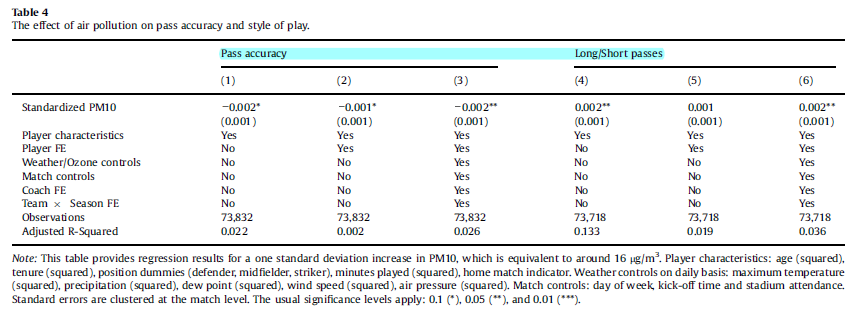
\includegraphics[scale = .7]{0522tanji_fig/t4}
    \label{t4}
  \end{figure}
\end{frame}

\begin{frame}\frametitle{}
  \begin{itemize}
    \item Pass accuracy
    \begin{itemize}
      \item Small but statistically significant negative effect was found:
      \begin{itemize}
        \item One standard deviation increase in PM10 concentration reduces pass accuracy by around .2\%.
      \end{itemize}
    \end{itemize}
    \item Ratio of long/short passes
    \begin{itemize}
      \item In response to air pollution, players adjust their style of play:
      \begin{itemize}
        \item Players reduce the ratio of short passes to avoid physical strain.
      \end{itemize}
    \end{itemize}
  \end{itemize}
\end{frame}

\begin{frame}\frametitle{Effect heterogeneity}
  \begin{figure}
    \centering
    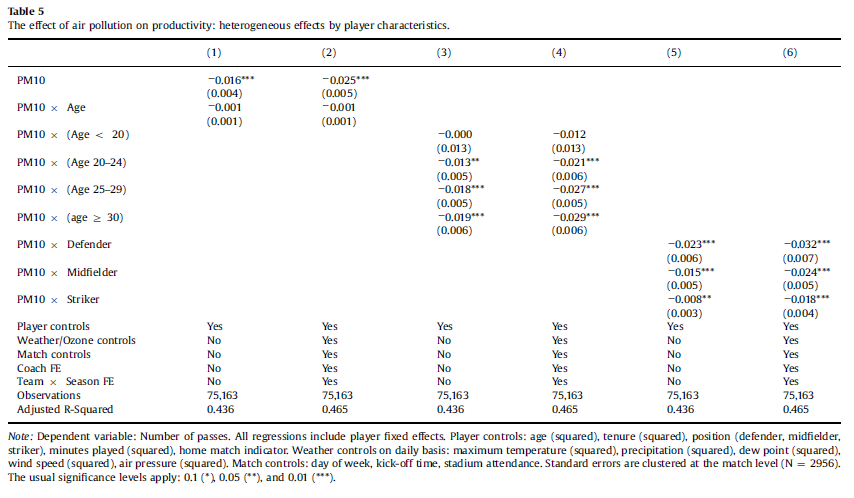
\includegraphics[scale = .7]{0522tanji_fig/t5}
    \label{t5}
  \end{figure}
\end{frame}

\begin{frame}\frametitle{}
  \begin{itemize}
    \item Professional soccer players constitute a rather homogeneous group that is positively selected w.r.t. their overall physical condition.
    \item Even so, there are heterogeneity of treatment effects with age:
    \begin{itemize}
      \item The productivity of the youngest group of players (age < 20) is not impaired by PM10, whereas all other players are negatively affected.
    \end{itemize}
    \item PM10 affects the productivity of all players irrespective of their position (except for goal keepers), but the defenders and midfielders are more effected than strikers.
  \end{itemize}
\end{frame}

\begin{frame}\frametitle{Effects of his team-mates and opponents}
  \begin{itemize}
    \item The productivity of a given player depends on that of his team-mates and his opponents.
    \item Team and match-level regression.
    \begin{itemize}
      \item The \# of match-level passes decreases statistically significantly with higher concentration of particulate matter.
      \item The \# of scored goals decrease at very high levels of pollution.
    \end{itemize}
    \item Pollution has a symmetrical effect on players.
  \end{itemize}
\end{frame}

\section{Conclusion}

\begin{frame}\frametitle{Concluding Remarks}
  \begin{itemize}
    \item Overall, their analysis complements previous empirical evidence on the negative effects of air pollution on the productivity.
    \item Even modetrate concentrations of particulate matter commonly experienced in developed countries impede the productivity of professional athletes to a considerable extent.
    \item \textbf{General the findings beyond the realm is not straight-forward.}
  \end{itemize}
\end{frame}

\end{document}
